\documentclass{article}

\usepackage[utf8]{inputenc}
\usepackage[spanish]{babel}

\usepackage{caratula}
\usepackage[toc,page]{appendix}
\usepackage{subcaption}
\usepackage{graphicx}
\usepackage{dirtytalk}
\usepackage{enumerate}

\usepackage{amssymb}
\usepackage{mathtools}
\usepackage{amsmath}
\usepackage{amsthm}

\usepackage{algorithm}
\usepackage{algpseudocode}
\usepackage{listingsutf8}

\usepackage{float}
\floatplacement{figure}{h!}

\usepackage{geometry}
\usepackage{fixltx2e}
\usepackage{wrapfig}
\usepackage{cite}
\usepackage{dsfont}
\usepackage{ulem}

\usepackage[space]{grffile}

\geometry{
 a4paper,
 total={210mm,297mm},
 left=30mm,
 right=30mm,
 top=20mm,
 bottom=20mm,
 }

\usepackage{booktabs}

% sql stuff
\usepackage{listings}
\usepackage{courier}
\usepackage{pdflscape}

\newcommand\JSONnumbervaluestyle{\color{blue}}
\newcommand\JSONstringvaluestyle{\color{red}}

% switch used as state variable
\newif\ifcolonfoundonthisline

\makeatletter

\lstdefinestyle{json}
{
  showstringspaces    = false,
  keywords            = {false,true},
  alsoletter          = 0123456789.,
  morestring          = [s]{"}{"},
  stringstyle         = \ifcolonfoundonthisline\JSONstringvaluestyle\fi,
  MoreSelectCharTable =%
    \lst@DefSaveDef{`:}\colon@json{\processColon@json},
  basicstyle          = \ttfamily,
  keywordstyle        = \ttfamily\bfseries,
}

% flip the switch if a colon is found in Pmode
\newcommand\processColon@json{%
  \colon@json%
  \ifnum\lst@mode=\lst@Pmode%
    \global\colonfoundonthislinetrue%
  \fi
}

\lst@AddToHook{Output}{%
  \ifcolonfoundonthisline%
    \ifnum\lst@mode=\lst@Pmode%
      \def\lst@thestyle{\JSONnumbervaluestyle}%
    \fi
  \fi
  %override by keyword style if a keyword is detected!
  \lsthk@DetectKeywords%
}

% reset the switch at the end of line
\lst@AddToHook{EOL}%
  {\global\colonfoundonthislinefalse}

\newtheorem{theorem}{Teorema}[section]
\newtheorem{corollary}{Corolario}[theorem]
\newtheorem{lemma}{Lema}[theorem]

\theoremstyle{definition}
\newtheorem{definition}{Definición}[section]

\theoremstyle{remark}
\newtheorem*{remark}{Observación}

\usepackage[dvipsnames]{xcolor}

% table of contents depth
\setcounter{tocdepth}{3}

\begin{document}
% Estos comandos deben ir antes del \maketitle
\materia{Ingeniería de Software II} % obligatorio

\titulo{TP2}
\subtitulo{Alerta y Vigliancia de Yacimientos Semi-Automático \\ \textbf{AVYSA} \\ \today}
\grupo{}

\integrante{Christian Cuneo}{755/13}{chriscuneo93@gmail.com}
\integrante{Federico Beuter}{827/13}{federicobeuter@gmail.com}
\integrante{Mauro Cherubini}{835/13}{cheru.mf@gmail.com}
\integrante{Mario Ezequiel Ginsberg}{145/14}{ezequielginsberg@gmail.com}
\integrante{Martín Baigorria}{575/14}{martinbaigorria@gmail.com}

\maketitle

\tableofcontents

\vspace{2cm}

\begin{figure}[H]
    \centering
    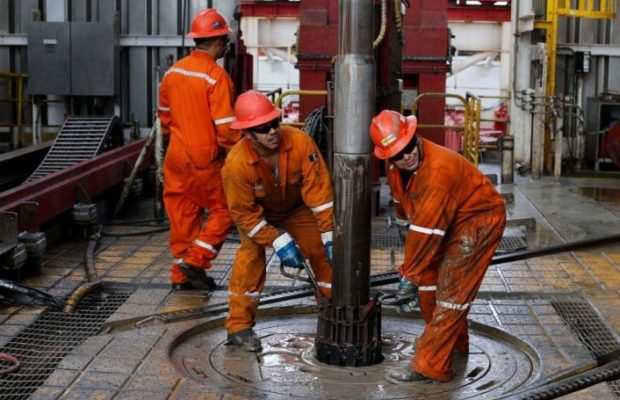
\includegraphics[scale=0.6]{figures/trabajadores.jpg}
    \caption{Trabajadores arreglando un problema diagnosticado mediante el sistema ARS luego del segundo recuperatorio.}
\end{figure}

\pagebreak

\section{Introducción}

Luego de desarrollar el simulador SimOil, aprovechando que ya habíamos adquirido el conocimiento de dominio de la industria petrolera, el Ministerio de Energía se ha mostrado interesado en integrar dicho sistema de simulación al sistema de control de pozos inteligentes que posee la empresa petrolera estatal. Este sistema monitorea el flujo producido, el flujo de reinyección de gas/agua, las presiones y las temperaturas por pozo. De esta manera, se pueden diagnosticar problemas y gestionar mejor los recursos de cada yacimiento. La tecnología de pozos inteligentes utiliza una serie de sensores ubicados en cada pozo, que reportan datos de alta frecuencia. Dado el gran volumen de datos, los ingenieros requieren un sistema diseñado especialmente para identificar cualquier tipo de inconveniente a partir del estado de los pozos.

Para poder integrar el sistema SimOil al sistema de control de pozos inteligentes, la solución planteada busca en primer lugar reducir la dimensionalidad de los datos de alta frecuencia para que los mismos sean mas simples de procesar a través de un sistema automatizado de supervisión de yacimiento denominado ARS. El sistema ARS luego preparara los datos almacenados para que luego puedan ser utilizados por los diferentes ingenieros de forma remota. A grandes rasgos, el sistema consistirá en un pipeline de tres etapas:

\begin{figure}[H]
  \resizebox{\textwidth}{!}{
    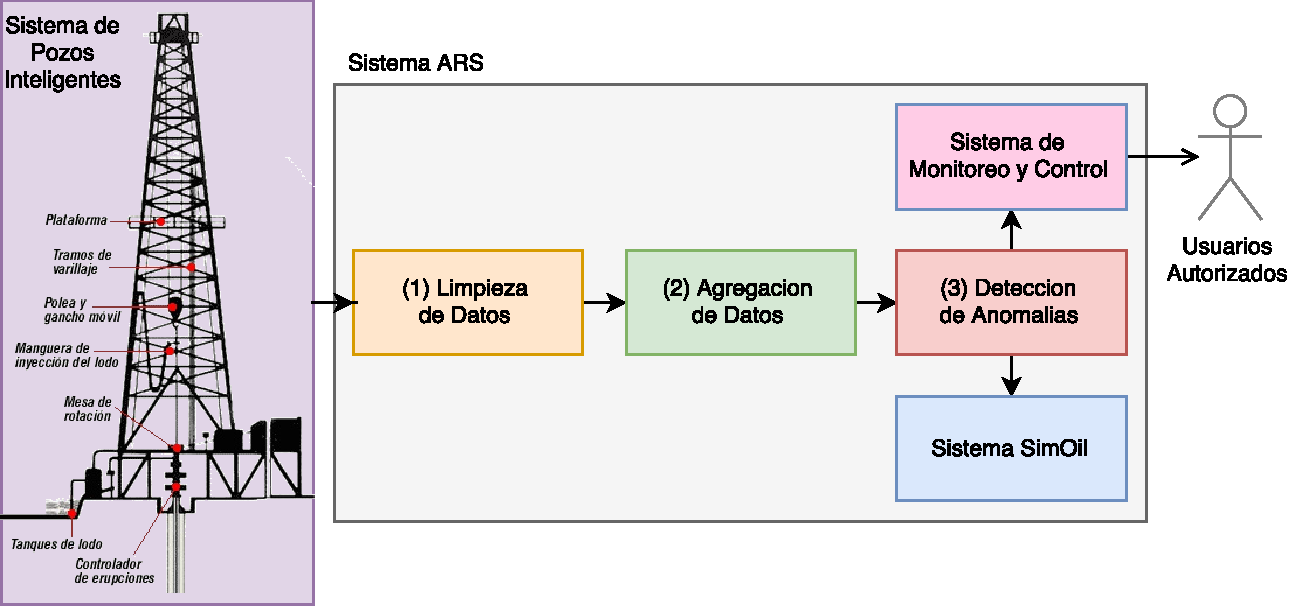
\includegraphics[scale=1]{figures/pipeline.pdf}
  }
  \caption{Esquema ilustrativo del sistema. El sistema de pozos inteligentes provee los datos de alta frecuencia a partir de sensores, que son procesados por el sistema ARS. A grandes rasgos, el sistema consiste en un pipeline de tres etapas, el cual luego provee datos a los usuarios autorizados a través del Sistema de Monitoreo y Control.}
\end{figure}

Cada uno de estos módulos del pipeline tiene las siguientes características:
\begin{enumerate}
  \item Limpieza de datos: Dado que los datos producidos por los sensores pueden no ser realistas, los mismos se filtran antes de comenzar con su correspondiente procesamiento. Los especialistas del dominio nos han confirmado que es posible identificar aproximadamente un 80\% de las anomalías utilizando limites superiores e inferiores para las diferentes medidas.
  \item Agregación de datos: El proceso de agregación transforma los datos de alta frecuencia en intervalos manejables de 15 minutos. Es razonable pensar que el estado de las variables de cada pozo es relativamente estable en intervalos lo suficientemente chicos, por lo que no tiene sentido procesar todas las mediciones de forma individual.
  \item Detección de anomalías: Utilizando los datos procesados y agregados, en conjunto con las simulaciones provistas por el sistema SimOil, es posible detectar problemas en pozos individuales utilizando algoritmos de Machine Learning. Las diferentes anomalías detectadas son luego reportadas al Jefe de Operaciones del respectivo yacimiento mediante SMS. Estos datos también están disponibles para que otros usuarios autorizados los consulten mediante una interfaz web.
\end{enumerate}

Al detectarse una anomalía, también se genera una alarma sonora en el centro de control del respectivo yacimiento donde sucedió el problema. Las alarmas pueden ser deshabilitadas de forma manual o mediante la interfaz del sistema ARS. Para que el sistema vuelva a operar de forma normal, el Jefe de Operaciones debe tomar una acción correctiva de ser necesaria o reportar un falso positivo de la alarma.

Dado que las normas internacionales son muy estrictas, se requiere que todos los registros de anomalías sean almacenados e informados a organismos certificadores de calidad, como el Ente Regulador de Seguridad Medio Ambiental (ERSMA). Los formularios de eventos deben estar disponibles para el Ministerio y para el Ente Regulador en todo momento. En cuanto a la accesibilidad de los datos y los reportes, el sistema también debe contar con perfiles de usuarios según sus cargos y responsabilidades.

El costo de construir un yacimiento petrolero es considerable. Cualquier decisión que no se tome de forma correcta puede tener un gran costo para el Ministerio. Por esta razón se considera que los datos son muy sensibles, haciendo necesario el almacenamiento de los mismos en un sitio seguro con un sistema de backup en caso de perdida o siniestro.

A modo de resumen, el ministerio ha puesto especial énfasis en las siguientes funcionalidades y atributos de calidad:
\begin{enumerate}
  \item Control de acceso diferenciado según el perfil del usuario.
  \item Tolerancia a fallas.
  \item Manejo de grandes volúmenes de datos.
  \item Seguridad a nivel de usuarios y acceso a datos.
  \item Gestión de las alarmas, formularios e informes de eventos críticos.
  \item Acceso al sistema de monitoreo y control desde el Ministerio.
  \item Acceso al sistema de informes de eventos críticos desde los entes reguladores.
  \item Toda la información estará centralizada dentro del Ministerio. El sistema no debe tener ningún tipo de demoras, en especial en las búsquedas de eventos, y debe tener una alta disponibilidad. Se debe buscar un mecanismo para que las consultas recurrentes sean rápidas. Esto podría implementarse mediante caching.
\end{enumerate}

\section{Casos de uso} \label{cu}

\subsection{Diagrama}

\begin{figure}[H]
    \centering
    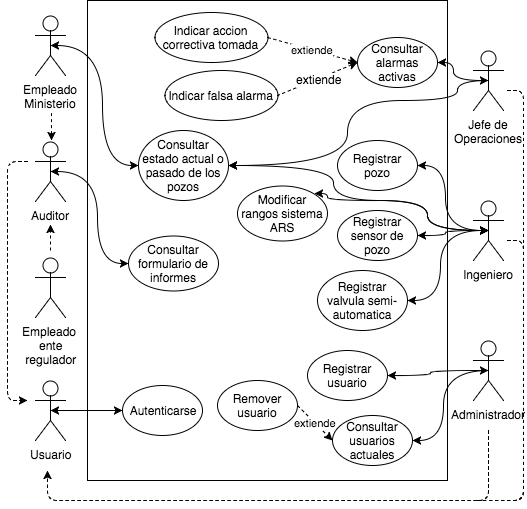
\includegraphics[width=0.7\textwidth]{figures/casosuso.png}
    \caption{Diagrama de casos de uso}
    \label{fig:casosuso}
\end{figure}

\subsection{Descripción}

\begin{enumerate}
    \item \textbf{Autenticándose}: La primera acción que tiene que realizar cualquier usuario, no importe su perfil, para poder seguir interactuando con el sistema con los permisos que tenga su perfil.
    \item \textbf{Registrando usuario}: La forma que tiene el administrador de ingresar un nuevo usuario al sistema, indicando el perfil que va a utilizar.
    \item \textbf{Removiendo usuario}: El administrador le saca el acceso al sistema a un usuario en particular.
    \item \textbf{Consultando usuarios actuales}: El administrador lista los usuarios actuales.
    \item \textbf{Registrando pozo}: De esta forma el ingeniero hace que el sistema considere un nuevo pozo en su procesamiento y lo agregue al simulador de simoil entre otras cosas.
    \item \textbf{Registrando sensor de pozo}: El ingeniero registra un nuevo sensor indicando el pozo al que pertenece para que el sistema sepa a que pozo pertenece.
    \item \textbf{Registrando válvula semiautomática}: El ingeniero registra una nueva válvula semiautomática indicando el pozo al que pertenece y su función.
    \item \textbf{Modificando rangos de sistema ARS}: Se modifican los rangos de limpieza de datos.
    \item \textbf{Consultando estado actual o pasado de los pozos}: Para consultar una historia de los valores de los sensores, posiciones de las válvulas y estados de alerta para cada pozo.
    \item \textbf{Consultando formulario de informes}: Se listan los informes detallados de eventos detectados por el sistema.
    \item \textbf{Consultando alarmas activas}: De esta forma el jefe de operaciones tiene acceso a las alarmas activas.
    \item \textbf{Indicando falsa alarma}: El jefe de operaciones cierra una alarma indicando que fue falsa alarma.
    \item \textbf{Indicando acción correctiva tomada}: El jefe de operaciones cierra una alarma indicando la acción correctiva tomada.
\end{enumerate}

\subsection{Especificación}

\newcommand{\curef}[1]{\textbf{Caso de uso \ref{cu:#1}}}
\newcommand{\cutitle}[1]{\renewcommand{\givencutitle}{#1}}
\newcommand{\cuactors}[1]{\renewcommand{\givencuactors}{#1}}
\newcommand{\cupre}[1]{\renewcommand{\givencupre}{#1}}
\newcommand{\cupost}[1]{\renewcommand{\givencupost}{#1}}
\newcommand{\cucourse}[1]{\renewcommand{\givencucourse}{#1}}
\newcommand{\culabel}[1]{\renewcommand{\givenculabel}{#1}}
\newcommand{\cucaption}[1]{\renewcommand{\givencucaption}{#1}}
\newcommand{\givencutitle}{REQUIRED!}
\newcommand{\givencuactors}{REQUIRED!}
\newcommand{\givencupre}{-}
\newcommand{\givencupost}{-}
\newcommand{\givencucourse}{REQUIRED!}
\newcommand{\givenculabel}{REQUIRED!}
\newcommand{\givencucaption}{} % optional

\newenvironment{casodeuso}
{\begin{table}[H]}{%
\begin{tabular}{|p{0.5\linewidth} p{0.5\linewidth}|}\hline
\multicolumn{2}{|l|}{\textbf{Caso de Uso: \ref{cu:\givenculabel}) \givencutitle}} \\
\multicolumn{2}{|l|}{\textbf{Actor:} \givencuactors} \\
\multicolumn{2}{|l|}{\textbf{Pre:} \givencupre} \\
\multicolumn{2}{|l|}{\textbf{Post:} \givencupost} \\
\vspace{1px}\textbf{Curso Normal} & \vspace{1px}\textbf{Curso Alternativo} \\
\givencucourse
\hline
\end{tabular}
\caption{\givencutitle}
\label{cu:\givenculabel}
\end{table}}

En esta sección identificaremos los tres casos de uso principales y los especificaremos en detalle utilizando la tabla de curso normal/alternativo.

\begin{casodeuso}
  \cutitle{Registrando válvula semiautomática}
  \cuactors{Ingeniero}
  \cupre{Ingeniero esta autenticado}
  \cupost{Válvula y su información queda registrada en el sistema para un poso especifico}
  \cucourse{
    1. El ingeniero selecciona la opción de ingresar una válvula & \\
    2. El sistema carga el listado de pozos actuales y sus válvulas \\
    3. El ingeniero selecciona un pozo al que corresponde la válvula & \\
    4. El sistema carga el listado de tipos de válvula & \\
    5. El ingeniero selecciona que tipo de válvula a ingresar & 5.1. La válvula del tipo seleccionado ya fue ingresada para ese pozo. Vuelve a 5. \\
    6. El ingeniero confirma selección & \\
    7. El sistema persiste la válvula & \\
    8. El sistema informa éxito de operación & \\
    9. Fin del caso & \\
  }
  \culabel{regval}
\end{casodeuso}

\begin{casodeuso}
  \cutitle{Indicando acción correctiva tomada}
  \cuactors{Jefe de operaciones}
  \cupre{Jefe de operaciones esta autenticado}
  \cupost{El evento queda cerrado junto con su informe}
  \cucourse{
    1. El jefe de operaciones selecciona la opción de indicar acción correctiva para la alarma seleccionada en la lista de alarmas activas & \\
    2. El sistema carga en detalle la alarma seleccionada & \\
    3. El jefe de operaciones indica de forma detallada la acción tomada & \\
    4. El jefe de operaciones confirma la operación & 4.1 Descripción es muy corta, vuelve a 3\\
    5. El sistema persiste la acción & \\
    6. El sistema completa el informe de la alarma & \\
    7. Fin del caso & \\
  }
  \culabel{indacc}
\end{casodeuso}

\begin{casodeuso}
  \cutitle{Consultando estado actual o pasado de los pozos}
  \cuactors{Empleado del ministerio, Ingeniero o Jefe de Operaciones}
  \cupre{El usuario esta autenticado y tiene el perfil correspondiente}
  \cupost{El usuario accedió a la información del estado de los pozos que necesitaba}
  \cucourse{
    1. El usuario selecciona la opción de listar los pozos & \\
    2. El sistema lista los pozos & \\
    3. El usuario selecciona el pozo a consultar & \\
    4. El sistema encuentra los registros de estados de válvulas para ese pozo & \\
    5. El sistema encuentra los registros de estados de sensores para ese pozo & \\
    6. El sistema encuentra los registros de alertas para ese pozo & \\
    7. El sistema muestra de forma detallada el historial y el estado actual de este pozo & \\
    8. Fin del caso & \\
  }
  \culabel{estact}
\end{casodeuso}

\pagebreak

\section{Atributos de calidad}

Antes de realizar la arquitectura, llevamos a cabo un Quality Attribute Workshop (QAW) para identificar los diferentes atributos de calidad requeridos. En nuestras reuniones con los stakeholders (consultas con el tutor), generamos, priorizamos y refinamos los diferentes atributos. Especificamos estos atributos de calidad mediante escenarios. La priorización final de los atributos de calidad que se acordó fue la siguiente:

\begin{enumerate}
  \item Performance
  \item Disponibilidad
  \item Seguridad
  \item Usabilidad
  \item Modificabilidad
\end{enumerate}

Para cada tipo de atributo de calidad definimos distintos escenarios de acuerdo a lo relevado.

\subsubsection{Performance}

1)
\begin{itemize}
  \item Descripción: La búsqueda de eventos en el sistema debe tardar a lo sumo medio segundo.
  \item Fuente: Auditor.
  \item Estímulo: Escribe en el buscador el evento a buscar y aprieta el botón Buscar.
  \item Artefacto: Sistema de Monitoréo y Control.
  \item Entorno: Normal.
  \item Respuesta: Se obtienen los datos del evento buscado. Si la búsqueda es idéntica a otra realizada hace menos de 1 hora, la respuesta llegará más rápido.
  \item Medición: El sistema responderá la búsqueda en menos de 100 ms en el caso de una búsqueda repetida recientemente, y en menos de 500 ms en cualquier otro caso.
\end{itemize}

2)
\begin{itemize}
  \item Descripción: La limpieza de datos deberá remover aproximadamente el 80\% de los picos no realistas del conjunto de datos.
  \item Fuente: Interna. % ó Ingeniero
  \item Estímulo: Llegan nuevos datos a ser limpiados de datos no realistas. % ó Selecciona el conjunto de datos a limpiar y  \item aprieta el botón Limpiar.
  \item Artefacto: Sistema de Procesamiento de Mediciones. % ó Sistema de Monitoreo y Control.
  \item Entorno: Normal.
  \item Respuesta: El sistema realiza la limpieza de datos correctamente.
  \item Medición: Aproximadamente el 80\% de los picos fuera de los límites superior e inferior fueron eliminados del conjunto de datos.
\end{itemize}

3)
\begin{itemize}
  \item Descripción: La detección de anomalías no debe tardar más de 5 minutos.
  \item Fuente: Interna.
  \item Estímulo: Llegan nuevos datos anómalos a ser analizados.
  \item Artefacto: Detector de Anomalías.
  \item Entorno: Normal.
  \item Respuesta: Se detectan las anomalías y se da aviso al Gestor de Anomalías.
  \item Medición: Las anomalías son detectadas en menos de 5 minutos.
\end{itemize}

\pagebreak

4)
\begin{itemize}
  \item Descripción: Ante un pronóstico catastrófico, la alarma debe ser enviada inmediatamente.
  \item Fuente: Interna.
  \item Estímulo: Evento catastrófico detectado por el módulo Detector de Anomalías.
  \item Artefacto: Gestor de Anomalías.
  \item Entorno: Normal.
  \item Respuesta: Envío inmediato de SMS al Jefe de Operaciones del yacimiento.
  \item Medición: El SMS se envía en menos de 1 segundo.
\end{itemize}

\subsubsection{Disponibilidad}

1)
\begin{itemize}
  \item Descripción: El sistema de procesamiento de mediciones debe estar en funcionamiento todo el tiempo para garantizar la mayor efectividad de detección de catástrofes.
  \item Fuente: Interna.
  \item Estímulo: Llegan datos a ser analizados.
  \item Artefacto: Sistema de Procesamiento de Mediciones.
  \item Entorno: Degradado.
  \item Respuesta: Otra instancia del procesador de mediciones se encarga de procesar los datos.
  \item Medición: En el 99.999\% de los casos los datos se procesaron correctamente.
\end{itemize}

2)
\begin{itemize}
  \item Descripción: El formulario de eventos debe estar disponible en todo momento para el Ministerio y para el Ente Regulador de Seguridad Medio Ambiental.
  \item Fuente: Externa.
  \item Estímulo: Petición para visualizar el formulario de eventos.
  \item Artefacto: Sistema de Informes de Eventos.
  \item Entorno: Degradado.
  \item Respuesta: El balanceador de carga asigna otro sistema de informes de eventos para realizar la petición.
  \item Medición: En el 99.999\% de los casos los datos se visualizaron correctamente.
\end{itemize}

3)
\begin{itemize}
  \item Descripción: El sistema en su totalidad debe ser tolerante a fallas.
  \item Fuente: Interna.
  \item Estímulo: Un módulo del sistema deja de funcionar.
  \item Artefacto: Sistema.
  \item Entorno: Normal.
  \item Respuesta: El sistema omite el módulo degradado.
  \item Medición: El sistema sigue en funcionamiento.
\end{itemize}

\pagebreak

4)
\begin{itemize}
  \item Descripción: El servicio de envío de SMS debe estar siempre en funcionamiento.
  \item Fuente: Externa.
  \item Estímulo: Se recibe un mensaje de error de envío de SMS.
  \item Artefacto: Gestor de Anomalías.
  \item Entorno: Normal.
  \item Respuesta: Se envía nuevamente el SMS por otro canal de envío de SMS.
  \item Medición: Se recibe una confirmación de envío del mensaje en menos de 1 segundo.
\end{itemize}

5)
\begin{itemize}
  \item Descripción: En caso de siniestro, todos los registros deben mantenerse accesibles.
  \item Fuente: Interna.
  \item Estímulo: Se desea acceder a un registro.
  \item Artefacto: Gestor de Anomalías.
  \item Entorno: Degradado.
  \item Respuesta: El sistema redirige la petición al Gestor de Backups.
  \item Medición: Los datos son obtenidos en el 99.999\% de las veces.
\end{itemize}

\subsubsection{Seguridad}
1)
\begin{itemize}
  \item Descripción: La autenticación de los usuarios debe ser segura.
  \item Fuente: Agente Externo.
  \item Estímulo: Un agente externo intenta interceptar los datos de un usuario cuando son enviados al sistema para el logueo en el mismo.
  \item Artefacto: Sistema de Usuarios.
  \item Entorno: Normal.
  \item Respuesta: Los datos se envían de forma segura.
  \item Medición: Debido al método de seguridad usado para enviar los datos, en menos del 0.00000001\% de los casos el agente externo logra descifrar los datos en menos de 1 semana.
\end{itemize}

2)
\begin{itemize}
  \item Descripción: Los datos de los servicios externos se deben recibir de forma segura.
  \item Fuente: Agente Externo.
  \item Estímulo: Un agente externo intenta interceptar los datos de los servicios externos cuando son enviados al sistema para  el procesamiento de los mismos.
  \item Artefacto: Controlador de válvula semiautomática.
  \item Entorno: Normal.
  \item Respuesta: Los datos son recibidos de forma segura.
  \item Medición: Debido al método de seguridad usado para enviar los datos, en menos del 0.00000001\% de los casos el agente externo logra descifrar los datos en menos de 1 semana.
\end{itemize}

\pagebreak

3)
\begin{itemize}
  \item Descripción: Un determinado perfil de usuario sólo puede ejecutar las acciones permitidas por dicho perfil.
  \item Fuente: Usuario. %Ingeniero. (pongo un ejemplo concreto, pero serviría para cualquier rol que intente hacer algo que no debería, no sé si está bien con esa descripción general poner roles particulares)
  \item Estímulo: Intenta realizar una acción para la cual no está autorizado su perfil.
  \item Artefacto: Sistema.
  \item Entorno: Normal.
  \item Respuesta: El sistema invalida la acción y muestra un mensaje de error indicando la incompatibilidad de la acción con el perfil del usuario.
  \item Medición: Solo al probar una pagina a la que el cada tipo de usuario no debe tener acceso el sistema muestra un mensaje de error.
\end{itemize}

\subsubsection{Usabilidad}
1)
\begin{itemize}
  \item Descripción: El sistema debe ser fácil de aprender a usar y agradable a la vista.
  \item Fuente: Usuario.
  \item Estímulo: Interactúa con el sistema.
  \item Artefacto: Interfaz de Usuario.
  \item Entorno: Ejecución.
  \item Respuesta: Responde con mensajes claros y precisos, y muestra de forma simple y elegante las distintas acciones posibles dentro del sistema.
  \item Medición: Cualquier usuario debe poder aprender a usar el sistema en menos de 10 minutos.
\end{itemize}

\subsubsection{Modificabilidad}
1)
\begin{itemize}
  \item Descripción: El sistema debe poder permitir el agregado de nuevos procesos para trabajar con los datos almacenados sin mucha dificultad.
  \item Fuente: Desarrollador.
  \item Estímulo: Quiere agregar un nuevo proceso.
  \item Artefacto: Sistema.
  \item Entorno: En diseño.
  \item Respuesta: Se realizan los cambios sin afectar las otras funcionalidades.
  \item Medición: Se agregó el nuevo proceso modificando sólo 2 módulos.
\end{itemize}

\pagebreak

\section{Arquitectura}

\subsection{Diagrama general}

\begin{figure}[H]
  \centerline{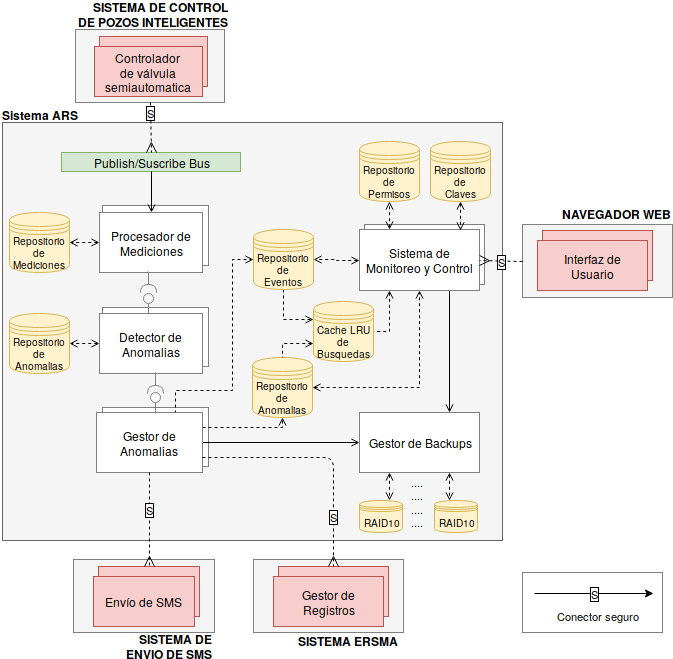
\includegraphics[scale=0.8]{figures/architecture.png}}
  \caption{Diagrama general de la arquitectura del sistema ARS de supervisión automática de yacimientos.}
\end{figure}

\pagebreak

La arquitectura del Sistema ARS busca procesar los datos de alta frecuencia que son producidos por los diferentes controladores de válvula semiautomática del Sistema de Control de Pozos Inteligentes (SCPO). Cada controlador publica las mediciones de la válvula en un Publish/Suscribe Bus al que esta suscripto el componente de Procesamiento de Mediciones. El Procesador de Mediciones (sección \ref{procesador_mediciones}) básicamente se ocupa de transformar los datos de forma tal que puedan ser consumidos por el Detector de Anomalías. Notar que los datos llegan a los procesadores de mediciones de forma asíncrona, el emisor no se bloquea. Dada la gran cantidad de datos, procesar todas las mediciones sin perdidas es sumamente complejo. Por esta razón, se decidió llevar a cabo un proceso de sampling aleatorio. Aprovechando que las mediciones consecutivas de cada controlador en general no cambian, los procesos funcionan utilizando toda su capacidad aunque perdiendo algunas mediciones. El matemático de nuestro equipo ha mostrado que dada la frecuencia de las mediciones por controlador, existe un numero procesos necesarios en función de la cantidad de controladores conectados al sistema tal que la perdida de información converge a cero. Dada cierta tolerancia, este numero de procesos no es prohibitivo dada las características del hardware disponible en la actualidad.

Una vez preprocesadas las mediciones, dado que la dimensionalidad de las mismas ahora es considerablemente menor, pueden ser enviadas mediante un pipe al Detector de Anomalías. El Detector de Anomalías (sección \ref{detector_anomalias}) identifica las diferentes anomalías en las mediciones, que son consumidas por el Gestor de Anomalías (sección \ref{gestor_anomalias}). Este componente notifica por SMS al Jefe de Operaciones del yacimiento cuando se produce una anomalía y guarda diferentes registros en los Repositorios de Eventos y de Anomalías. El componente también se comunica con un Gestor de Backups mediante un call asincrónico (no bloqueante) para garantizar la integridad de los datos ante casos de perdida o siniestros. Para cumplir con las normas internacionales, toda anomalía también es reportada a los organismos certificadores de calidad como el Ente Regulador de Seguridad Medio Ambiental (ERSMA).

Utilizando los datos que el Gestor de Anomalías guarda en el Repositorio de Eventos y el Repositorio de Anomalías, el Sistema de Monitoreo y Control (sección \ref{monitoreo_y_control}) provee diferentes servicios a los usuarios autorizados, sean los ingenieros de cada yacimiento, los encargados de las auditorías del ERSMA o el jefe de operaciones. Estos usuarios primero deben ser autenticados mediante el uso de un usuario y una clave.

El Sistema de Monitoreo y Control también se comunica de forma asíncrona con el Gestor de Backups para realizar un backup incremental de cualquier cambio realizado a los repositorios de Eventos y Anomalías. También es posible hacer un backup de los repositorios con información de los usuarios.

Dado que el Ministerio de Energía estaba sumamente interesado en que las búsquedas de eventos funcionen rápido, y considerando que en general es mas probable que las ultimas consultas realizadas se repitan, decidimos agregar una cache LRU para el Repositorio de Eventos y el de Anomalías.

Para garantizar la confidencialidad de los datos, toda comunicación con un sistema externo es cifrada usando algoritmos simétricos (SMS y sistema ERSMA) y de clave publica/privada (otros usuarios).

\subsection{Procesamiento de mediciones}  \label{procesador_mediciones}

\begin{figure}[H]
  \resizebox{\textwidth}{!}{
    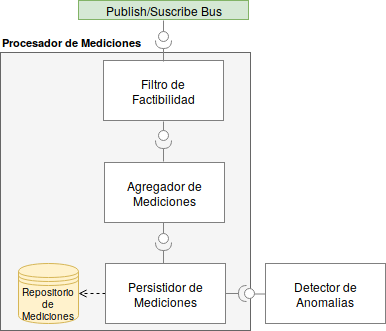
\includegraphics[scale=0.70]{figures/ProcesadorDeMediciones.png}
  }
  \caption{Diagrama de arquitectura de procesamiento de mediciones.}
\end{figure}

El Procesador de Mediciones consume datos de los diferentes controladores de válvula semiautomática de cada pozo a través de un Publish/Suscribe bus con calls asincrónicos. Como hemos explicado en la sección anterior, dada la alta frecuencia de los datos, hacemos sampling con una cierta cantidad de procesos para no perder información. En una primera etapa, no es factible ni practico hacer un backup de todos los datos antes de comenzar su procesamiento. Para reducir la cantidad de datos, primero se corre un Filtro de Factibilidad para remover los datos que no son realistas. Este filtro logra remover el 80\% de los datos espurios. Luego, los datos son agregados por el Agregador de Mediciones, el cual transforma los datos de alta frecuencia en datos en intervalos manejables de 15 minutos. Dado que tenemos muchos procesos que agregan mediciones y necesitan consultar el tiempo de forma recurrente, no queríamos que el Timer sea un bottleneck de este componente, por lo que también le dimos muchos procesos. Sin embargo, cabe destacar que los sistemas operativos modernos no necesitan muchos procesos de este tipo dado que en general se hace una lectura atómica desde un archivo. Estos datos son luego consumidos por un Persistidor de Mediciones, que guarda los datos procesados y de menor dimensionalidad en el Repositorio de Mediciones. Estos datos también son enviados por medio de una cola al Detector de Anomalías.

En caso de una caída del sistema, el Persistidor verifica si los datos en el Repositorio de Mediciones han sido reportados al Detector de Anomalías. En caso de que no, son enviados por el pipe. De todas maneras, dado que los datos son de alta frecuencia, podria no ser estrictamente necesario guardar un backup dado que las anomalías serán rápidamente reportadas al sistema nuevamente.

\subsection{Detector de anomalías} \label{detector_anomalias}

\begin{figure}[H]
  \resizebox{\textwidth}{!}{
    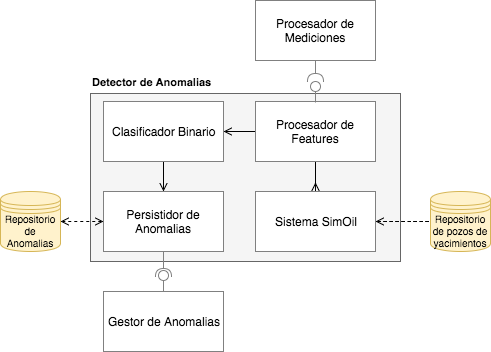
\includegraphics[scale=0.8]{figures/DetectorDeAnomalias.png}
  }
  \caption{Diagrama de arquitectura del detector de anomalías.}
\end{figure}

El Detector de Anomalías procesa los datos provistos por el Persistidor de Mediciones, arrancando con el Procesador de Features. Este componente extrae una serie de features o características a partir de las mediciones con la asistencia del Sistema SimOil especificado en el trabajo anterior. Una vez procesados estos datos, se utiliza un clasificador binario (por el momento un modelo Logístico que ya esta entrenado) para definir si el dato procesado es o no una anomalía. Para definir si la observación es una anomalía o no, el clasificador binario requiere de un threshold. La idea es calibrar este threshold de forma tal que se minimicen los falsos negativos, dado que es mas grave no enterarse de una anomalía que una falsa alarma. Cuando el clasificador identifica una posible anomalía, se envía al Persistidor de Anomalías para bajar la probabilidad de perdida de datos ante un problema del sistema. En caso de una falla, al reiniciarse el proceso se verifica si hay datos en el Repositorio de Anomalías que no han sido enviados al Gestor de Anomalías.

\subsection{Gestor de anomalias} \label{gestor_anomalias}

\begin{figure}[H]
  \resizebox{\textwidth}{!}{
    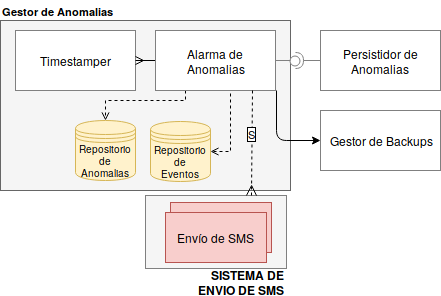
\includegraphics[scale=1]{figures/GestorDeAnomalias.png}
  }
  \caption{Diagrama de arquitectura del Gestor de Anomalías.}
\end{figure}

Al recibir datos de anomalías detectadas desde el Persistidor de Anomalías, la Alarma de Anomalías se ocupa de notificar al Jefe de Operaciones del correspondiente yacimiento de que se ha producido una anomalía. También se envía el registro al Sistema del ERSMA. Estas dos conexiones externas se hacen utilizando un cifrado de clave simétrica, cuya clave podría estar en un repositorio o hardcodeado en la misma alarma. A los datos luego se les asigna un timestamp y son guardados en el Repositorio de Anomalías y en el Repositorio de Eventos. Para lograr una mayor disponibilidad y tener un sistema tolerante a fallas, los datos de anomalías también son enviados a un Gestor de Backups mediante un call asincronico. En caso de falla, los procesos del componente se reinician y buscan los datos sobre las ultimas fallas que han ocurrido y no han sido reportadas desde este repositorio.

\subsection{Sistema de Monitoreo y Control} \label{monitoreo_y_control}

\begin{figure}[H]
 \resizebox{\textwidth}{!}{
    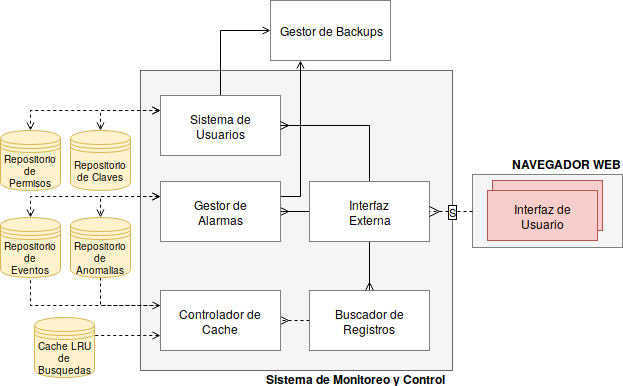
\includegraphics[scale=1]{figures/SistemaDeMonitoreoYControl.png}
  }
  \caption{Diagrama de arquitectura del Sistema de Monitoreo y Control.}
\end{figure}

El Sistema de Monitoreo y control se ocupa de dar una interfaz unificada para los usuarios externos del sistema, sean ingenieros, el jefe de operaciones o empleados del ERSMA. El mismo provee un control de acceso diferenciado según el tipo de usuario mediante el Sistema de Usuarios y los repositorios de Permisos y de Claves.

Al suceder una alarma, el Jefe de Operaciones del yacimiento puede ingresar al sistema con su login y luego gestionar las alarmas mediante el Gestor de Alarmas. De esta manera el Jefe de Operaciones puede tomar una acción correctiva o reportar un falso positivo de la alarma. Al tomar una decisión se completa el informe correspondiente a la anomalía en el Repositorio de Eventos.

Tomando en cuenta que el ministerio nos ha dicho que toda búsqueda realizada por un usuario se realiza nuevamente con una alta probabilidad, agregamos un Controlador de Cache entre el Buscador de Registros y los repositorios de Eventos y Anomalías para acelerar el tiempo de respuesta de las consultas.

\begin{figure}[H]
 \resizebox{\textwidth}{!}{
    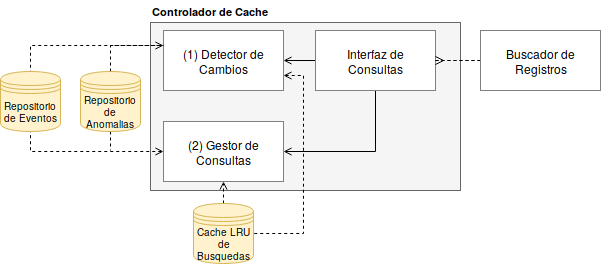
\includegraphics[scale=1]{figures/ControladorDeCache.png}
  }
  \caption{Diagrama de arquitectura del Controlador de Cache.}
\end{figure}

En una primera etapa, el controlador de cache debe verificar que los datos guardados en la cache siguen siendo vigentes. El Detector de Cambios consulta algún tipo de identificador único de consulta (un hash) de la Cache LRU que satisface la consulta (se podría agregar un componente que haga hashes, no lo consideramos necesario). Luego de alguna manera verifica que no se han realizado cambios en los repositorios de Eventos y Anomalías con una consulta rápida. En caso de que se hayan realizado cambios, se le comunica al Gestor de Consultas de que debe realizar la consulta desde los repositorios de Eventos y Anomalías. Caso contrario, toma los datos de la Cache. Los calls sincrónicos se podrían hacer de (1) a (2) y luego el resultado se podría reportar a la interfaz de consultas. A nivel arquitectura, se podría asumir a priori que la cache esta actualizada, y de forma asíncrona también consultar si se ha detectado un cambio para ganar mas velocidad. Sin embargo, si la detección de cambios es lo suficientemente rápida, esto agrega complejidad y no es necesario.

\pagebreak

\subsection{¿Como satisface la arquitectura los atributos de calidad?}

A continuación explicaremos de forma mas explicita como la arquitectura propuesta satisface los atributos de calidad, tomando como punto de partida los escenarios especificados en la Sección \ref{cu}.

\subsubsection{Performance}

\begin{enumerate}
  \item Como podemos ver en el diagrama general, el Sistema de Monitoreo y Control (SMyC) se encuentra replicado, permitiendo que se balancee la carga entre los mismos. Al no tener un balanceador de carga lo que se hace es que las interfaces de usuario se comuniquen aleatoriamente con un SMyC, balanceando la carga naturalmente. Además los SMyCs se comunican con un Cache de búsquedas, para no repetir las búsquedas iguales en un periodo corto de tiempo.
  \item El procesador de mediciones tiene un componente que se encarga de la limpieza de estos datos infactibles.
  \item Como se menciono previamente, entran datos al flujo constantemente, aunque se pierden unos pocos, se mantiene al sistema procesando al tope sin acumulación de mediciones, por lo tanto es prácticamente en tiempo real que son ingresados los actuales al flujo. Si bien por requerimientos los datos son agregados en intervalos manejables de 15 minutos, una vez que ese agregación es completada e ingresa al detector de anomalías el procesamiento es extremadamente rápido ya que la extracción de features es directa y luego.
  \item Apenas el detector de anomalías detecte un pronostico no animador va a comunicarse con el Gestor de Anomalías, el cual en su primer paso va a enviar el mensaje al jefe de operaciones a través de algún sistema de envió de SMS que se pide como requerimiento que tenga una disponibilidad de 99.99\% y un retraso máximo de 100ms.
\end{enumerate}

\subsubsection{Disponibilidad}

\begin{enumerate}
  \item Al tener un bus y replicado el componente podemos garantizar que siempre habrá alguno disponible para procesar nuevos datos publicados.
  \item Al tener replicado el Sistema de Monitoreo y Control la interfaz puede intentar comunicarse con otra instancia hasta que haya una que responda. Además la interfaz puede siempre elegir aleatoriamente la instancia a la cual comunicarse, garantizando naturalmente un balanceo correcto de la carga.
  \item Al tener replicado los componentes internos del sistema, ante la falla de uno el flujo se va poder continuar a través de otros, sin afectar la integridad general del sistema.
  \item Se va a intentar enviar el mensaje por algún servicio de SMS, si este no responde dentro de los 100ms requeridos se puede intentar en el resto de los servicios de SMS. Como el atributo indica un máximo de un segundo, son aproximadamente 10 intentos alternando el proveedor de servicio, lo cual es bastante robusto.
  \item Como explicamos anteriormente, al enviarse siempre las anomalías al Gestor de backups, estarán disponibles al reiniciarse el servicio en caso de una falla para podes atender anomalías no atendidas previamente.

\end{enumerate}

\subsubsection{Seguridad}

\begin{enumerate}
  \item Al estar usando un conector seguro, se esta utilizando un esquema de seguridad utilizado en la actualidad de forma masiva, y garantizado por el tiempo que a estado en uso sin que haya sido quebrado en un tiempo útil para un atacante.
  \item Nuevamente lo del punto anterior. Pero agregando que el sistema no contempla que se manipulen directamente los sensores y que estos envíen datos manipulados al sistema aunque creemos que esta debe ser una garantía de los sensores y no se encuentra dentro de lo que puede controlar nuestro sistema ya que seria una solución mas física que otra cosa.
  \item Para esto hay un sistema de usuarios dedicado a manejar permisos, a este sistema se conecta directamente la Interfaz Externa, que es el único punto de entrada que se tiene al sistema, controlando totalmente las acciones realizadas sobre el mismo.
\end{enumerate}

\subsubsection{Usabilidad}

\begin{enumerate}
  \item Si bien en esta clase de diagramas de diseño no se puede garantizar este atributo, la interfaz externa propuesta permite implementar una gama flexible de interfaces de usuario finales atractivas y fáciles de usar.
\end{enumerate}

\subsubsection{Modificabilidad}

\begin{enumerate}
  \item Trabajar con los datos almacenados simplemente no va a generar cambios drásticos, ya que simplemente se van a tener que compartir los repositorios correspondiente, como mucho teniendo que modificar los componentes actuales que se comunican con ellos, aunque si se implementa pensando en esto desde un principio, los repositorios podrían implementarse desde el vamos con posibilidad de compartirse, solucionando a futuro esta inquietud.
\end{enumerate}

\pagebreak

\section{Conclusiones}

Durante estos dos trabajos prácticos vimos distintos enfoques a la hora de diseñar software. Durante el primer trabajo utilizamos el diseño orientado a objetos (DOO), lo cual nos permitió realizar un diseño de más bajo nivel que el concebido mediante las diferentes arquitecturas del sistema (vista de C\&C + deployment). Con el DOO (programming in the small) pudimos diseñar reconociendo las distintas entidades de nuestro dominio del problema y convertirlas en objetos que se relacionan entre sí mediante envíos de mensajes. De esta manera es muy fácil implementar nuestra aplicación y comenzar a trabajar sobre ella. Este enfoque tiene algunas desventajas ya que no podemos ver algunos detalles como por ejemplo dónde van a correr nuestros procesos.

Para poder ver más otros detalles del sistema, entra en juego la arquitectura (programming in the large) que justamente viene a llenar ese vacío. La arquitectura nos permite ver las relaciones entre las distintas estructuras del sistema, y como se relacionan entre ellas, lo que resulta en una visión más abarcativa de la aplicación, no sólo porque nos permite definir las interacciones de nuestros procesos en tiempo de ejecución (mediante los diagramas de Componentes y Conectores) sino porque también nos permite identificar en dónde va a estar corriendo cada uno de esos procesos (mediante la vista de deployment).

Para concluir, el DOO es una muy buena forma de desarrollar módulos de la aplicación pero no es suficiente para desarrollar un buen sistema, ya que hay otro tipo de información relevante que no se puede visualizar con dichos módulos. Otra ventaja de las arquitecturas es que nos permite por medio de los escenarios de atributos de calidad proporcionarle al cliente un sistema que cumpla con los requerimientos no funcionales. Por esos motivos, es necesario construir arquitecturas usando el método de "programming in the large".

\end{document}
